\subsection{Struktur des REST-Service}

\subsubsection{Klassenstruktur}

Wie bereits erwähnt, ist die Aufgabe unseres REST-Service, eine Verbindung zwischen Benutzeranfragen und -eingaben auf der einen Seite und der Datenbank auf der anderen Seite herzustellen. Die Schnittstelle zur HTML-Kommunikation mit dem Benutzer bildet den REST-Service im engeren Sinne. Dieser wird bei uns von einer Klasse \texttt{Service} übernommen, in der wie zuvor beschrieben mit Jersey die REST-Schnittstelle implementiert wird. Die Kommunikation mit der Datenbank findet in der Klasse \texttt{Transactor} mittels JDBC statt.

Dabei gibt es jedoch keine direkte Kommunikation zwischen den Klassen \texttt{Service} und \texttt{Transactor}. Denn wie bereits in der Architekturübersicht dargestellt, besteht die Aufgabe des REST-Service im weiteren Sinne nicht nur in der Ausgabe von Daten aus der Datenbank, sondern auch aus deren Analyse. Zu diesem Analyseverfahren gehören das Clustering, die Identifikation von Peaks und die Darstellung von \textit{related news} sowie das Bestimmen von Einflussfaktoren des Sentiment-Wertes von Tweets. Damit diese Verfahren integriert werden können, befindet sich zwischen den \texttt{Service}- und \texttt{Transactor}-Klassen noch eine weitere Klasse \texttt{Logic}. Der Fluss der Daten sieht dabei folgendermaßen aus: eine REST-Anfrage des Benutzers ruft über Jersey die zugeordnete Methode der \texttt{Service}-Klasse auf. Diese Anfrage wird zunächst über die entsprechende Methode in \texttt{Logic} an eine \texttt{Transactor}-Methode weitergereicht, welche die benötigten Daten aus der Datenbank abruft. Diese werden dann an die \texttt{Logic}-Methode zurückgeliefert. Beinhaltet die Anfrage den Einsatz eines Analyseverfahrens, werden diese durch Einsatz der jeweils damit verbundenen Klassen an dieser Stelle durchgeführt. Wird beispielsweise das Clustering angefragt, liefert der \texttt{Transactor} eine entsprechende Auswahl Tweets, auf der dann in der \texttt{Logic}-Methode das Clustering durchgeführt wird.

Ein weiterer Aufgabenbereich der \texttt{Logic}-Klasse ist in einigen Fällen die Aufbereitung der vom \texttt{Transactor} zurückgelieferten Daten. Um beispielsweise den zeitlichen Verlauf der Aktivität oder des Meinungsbildes zu erhalten, werden von der Datenbank sämtliche Tweets nach der Stunde ihrer Erstellung gruppiert. Die Methode im Frontend, die diese Daten schlussendlich darstellen soll, erwartet dabei Paare aus Zeitpunkten und einer Anzahl in konstanten Intervallen. Da die Rückgabe der Datenbank die vollen Stunden, an denen gar keine Tweets erstellt wurden, gar nicht beinhaltet, müssen in der \texttt{Logic}-Klasse diese Zeitpunkte mit der Anzahl 0 nachträglich eingefügt werden.

Ist weder eine Analyse noch eine Aufbereitung der Daten notwendig, haben wir uns aus Gründen der Konsistenz der Implementierung entschieden, die \texttt{Logic}-Klasse nicht zu umgehen. In diesem Fall reicht sie die Ergebnisse einfach weiter.

Wie bereits im vorigen Kapitel angemerkt wurde, lassen sich mit Jersey sowohl Klassen als auch Methoden mit einem URL-Bestandteil versehen. Um eine semantische Trennung der REST-Anfragen zu gewährleisten, wurden auf diese Weise zwei REST-Service-Klassen implementiert. Die Klasse \texttt{ResultService} mit dem Pfadbestandteil \texttt{/results/} ist dabei für sämtliche Anfragen zuständig, welche mit den direkt für den Benutzer im Frontend sichtbaren Resultaten zu tun haben, d.\,h. den Inhalten der Views. Die Klasse \texttt{QueryService} mit dem Pfadbestandteil \texttt{/queries/} ist hingegen für alle übrigen internen Anfragen verantwortlich, wie zum Beispiel die Anfrage, ob ein spezifischer Suchbegriff bereits in der Datenbank vorhanden ist oder welche ID dieser hat. Analog dazu existieren die zwei \texttt{Logic}-Klassen \texttt{ResultLogic} und \texttt{QueryLogic}, welche allerdings weiterhin auf eine gemeinsame \texttt{Transactor}-Klasse zugreifen. Hintergrund dieser Trennung ist eine übersichtlichere Struktur sowohl der REST-API als auch des internen Java-Codes, welcher aufgrund der Vielzahl der Methoden ansonsten umständlich zu handhaben gewesen wäre.

\subsubsection{Data Transfer Objects}
\label{sec:dto}

Um die Kommunikation sowohl innerhalb des REST-Service als auch mit dem Frontend zu vereinfachen, haben wir uns für den Einsatz von \textit{Data Transfer Objects} (DTOs) entschieden. Dabei handelt es sich um ein \textit{Plain Old Java Object} (POJO), welches nur über private Felder sowie deren zugeordnete Getter und Setter verfügt. Da für gewöhnlich die Rückgabe einer Datenbankanfrage im Transactor sehr komplexe Daten mit einer großen Menge von Attributen zurückgibt, ist es sinnvoll, diese Daten in einem DTO zu kapseln, sodass sie leicht zu manipulieren sind und einfach zwischen Methoden verschickt werden können. Ein weiterer Vorteil ist, dass sich die DTOs unter Einsatz eines POJO-Mappers implizit ins JSON-Format parsen lassen, welches sich einfach in der JavaScript-Umgebung des Frontends verwenden und in Jersey als Rückgabetyp einer REST-Anfrage spezifizieren lässt.

Dies geschieht in unserem Projekt mithilfe der Bibliothek Jackson \cite{Jackson}. Diese stellt eine Reihe von Annotationen bereit, welche bei der Implementierung eines DTOs verwendet werden können, um festzulegen, wie dessen Attribute geparst werden sollen. Am wichtigsten sind dabei hier die Annotationen \texttt{@jsonproperty}, dessen Parameter festlegt, unter welchem Namen das Attribut im JSON geparst werden soll, sowie \texttt{@jsonignore}, das bestimmt, dass dieses Attribut beim Parsen ignoriert werden soll. Dabei können sämtliche primitiven Datentypen sowie alle Klassen, für die ebenfalls ein Jackson-Parsing definiert wurde, mit \texttt{@jsonproperty} versehen werden. Des Weiteren ist Jackson in der Lage, Arrays sowie Datenstrukturen mit direkter Entsprechung in JavaScript wie z.\,B. \texttt{List} oder \texttt{Map} in ihr JSON-Gegenstück zu parsen. Ein so über Jackson konfiguriertes DTO kann dann direkt im REST-Service als implizite HTML-Response an das Frontend zurückgeliefert werden, wo es im JSON-Format ankommt.

Auf diese Weise wurde für sämtliche Ressourcen ein geeignetes DTO implementiert. In einigen Fällen können dabei auch mehrere DTOs in einander geschachtelt sein. So sind zum Beispiel für die Darstellung eines Tweets im Frontend auch Informationen über den Benutzer notwendig, der diesen Tweet erstellt hat. Daher existiert ein DTO \texttt{TweetWithUser}, das wiederum die DTOs \texttt{Tweet} und \texttt{User} beinhaltet. Zusätzlich zu dieser Schachtelung von DTOs haben wir uns bei der Konzeption dafür entschieden, das Meta-DTO \texttt{Envelope} einzuführen, dass sämtliche anderen DTOs enthält. Der Vorteil eines solchen \texttt{Envelope} ist, dass es die Handhabung von Fehlern und anderem unerwarteten Verhalten ermöglicht. Zu diesem Zweck hat die Klasse neben dem Attribut \texttt{data} vom Typ \texttt{Object} zum Speichern des jeweiligen DTOs ebenfalls die Felder \texttt{status} und \texttt{error\_codes}. In \texttt{status} kann dabei der Erfolg der Operation abgespeichert werden (wobei in Anlehnung an HTML hauptsächlich \texttt{200 OK} für erfolgreiche Operationen und \texttt{500 Internal Server Error} für Fehler verwendet wurden), während \texttt{error\_codes} es ermöglicht, gegebenenfalls Informationen über die Fehlerursache wie z.\,B. die Stacktrace einer Exception zu hinterlegen. Da das \texttt{data}-Feld auch auf \texttt{null} belassen werden kann, kann in so einer Situation selbst dann ein Envelope zurückgeliefert werden, falls infolge eines Fehlers keine Daten vorliegen. Der Status sowie die Fehlernachricht ermöglichen dann das Abfangen von unerwartetem Verhalten im Frontend und erleichtern die anschließende Fehlerbehandlung.

Das Verpacken der DTOs geschieht dabei ebenfalls in der \texttt{Logic}-Klasse. Das bedeutet, dass das \texttt{ResultSet} der SQL-Anfrage im \texttt{Transactor} zunächst in einem DTO gekapselt wird, welches an die Methode in \texttt{Logic} übergeben wird. Unter Umständen geworfene Exceptions werden dabei ebenfalls zunächst unbehandelt weitergereicht. Wird in \texttt{Logic} eine Exception gefangen, liegen für gewöhnlich keine Daten vor, es wird dann ein \texttt{Envelope} mit negativem Status und der entsprechenden Stacktrace erstellt. Ansonsten wird das erhaltene DTO zusammen mit einem positiven Status in einen \texttt{Envelope} verpackt.

Die hier vorgestellte Struktur wird in Abbildung \ref{fig:reststruktur} visualisiert.

\begin{figure}[h]
\centering
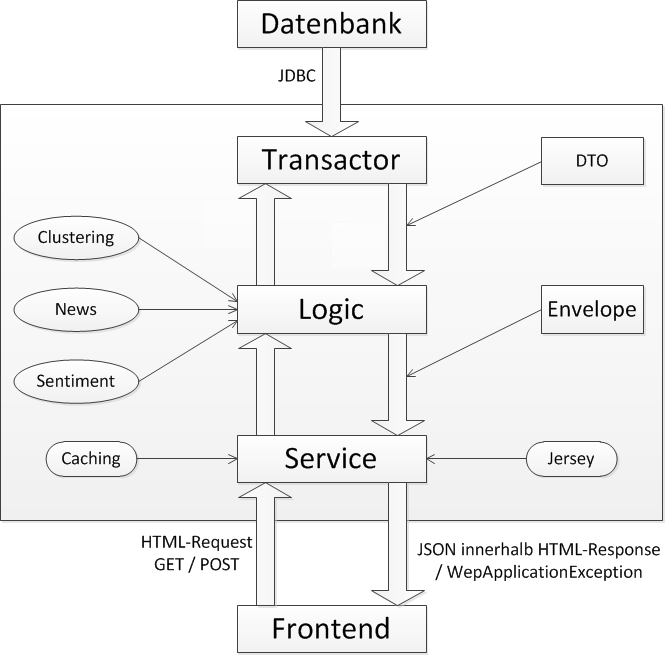
\includegraphics[width=0.6\textwidth]{Bilder/REST/RestServiceZeichnung.png}
\caption{Struktur des RestService}
\label{fig:reststruktur}
\end{figure}